\chapter{Policy Gradient Methods}
Recall the objective of Reinforcement Learning:
$$\theta = \argmaxA_\theta\mathbb{E}_{\tau\sim p_\theta(\tau)}\left[\sum_t r(s_t,a_t)\right]$$
This is actually framed as an optimization problem. Therefore, we can use a variety of optimization techniques, such as gradient descent, to optimize this objective. To be more concrete, let us define a function $J(\theta)$:
$$J(\theta) = \mathbb{E}_{\tau\sim \pi_\theta(\tau)}[r(\tau)]$$
By definition, $r(\tau)$ is the sum of reward incurred in this trajectory, so it can be equivalently defined as $\sum_{t=1}^T r(s_t,a_t)$, and by definition of expectation, we can more conveniently express the $J$ function as an integral of the product of policy and reward:
$$J(\theta) = \int \pi_\theta r(\tau)d\tau$$.
With this integral, we can easily take the gradient to perform gradient descent/ascent. A convenient expression of the gradient of $J(\theta)$ is shown below.
\section{Policy Gradient Theorem}
In this section, we will derive the mathematical expression of the policy gradient theorem.

Recall a convenient identity:
$$\pi_\theta(\tau)\nabla_\theta \log \pi_\theta(\tau) = \pi_\theta(\tau)\frac{\nabla_\theta \pi_\theta(\tau)}{\pi_\theta(\tau)}=\nabla \pi_\theta (\tau)$$
Using this identity, we can take the gradient of $J(\theta)$ in a cleaner fashion:
\begin{align*}
\nabla_\theta J(\theta) = \int \nabla_\theta \pi_\theta r(\tau)d\tau\\
=\int\pi_\theta(\tau)\nabla_\theta \log \pi_\theta(\tau) r(\tau) d\tau\\
= \mathbb{E}_{\tau\sim \pi_\theta(\tau)}[\nabla \log \pi_\theta (\tau)r(\tau)]
\end{align*}
Now, we want to get rid of the huge $\log \pi_\theta(\tau)$ from our equation. Recall that a trajectory $\tau$ is a list of states and actions, so $\pi_\theta(s_1,a_1,...,s_T,a_T) = p(s_1)\prod_{t=1}^T\pi_\theta (a_t|s_t)p(s_{t+1}|s_t,a_t)$ by Baye's rule. Then we take the log on both sides, and we end up getting $\log\pi_\theta(\tau) = \log p(s_1) + \sum_{t=1}^T \log\pi_\theta(a_t|s_t)+\log p(s_{t+1}|s_t,a_t)$.
Plugging into our original gradient:
\begin{equation}
\begin{aligned}
    \nabla_\theta J(\theta) &= \mathbb{E}_{\tau\sim \pi_\theta(\tau)}\left[\nabla_\theta\left(\log p(s_1) + \sum_{t=1}^T \log \pi_\theta(a_t|s_t)+\log p(s_{t+1}|s_t,a_t)\right)r(\tau)\right]\\
    &= \mathbb{E}_{\tau\sim \pi_\theta(\tau)}\left[ \left(\sum_{t=1}^T\nabla_\theta \log\pi_\theta(a_t|s_t)\right)\left(\sum_{t=1}^T r(s_t,a_t)\right)\right]
\end{aligned}
\end{equation}
Note that in the above calculation, we cancel out $\log p(s_1)$ and $\log p(s_{t+1}|s_t,a_t)$ because we are taking the gradient with respect to $\theta$, but those two expressions do not depend on $\theta$. The first item in the final expectation is similar to maximum likelihood.
\section{Evaluating the Policy Gradient}
In our derivation, we mathematically derived an expression for policy gradient. However, in most cases we cannot easily obtain the expectation easily because it is highly possible to involve a huge integral. Therefore, what are we going to do if the expectation (integral) is hard to evaluate? The answer is to approximate, and more specifically, we use Monte Carlo approximation. The idea is to take N samples, and average them out:
$$\nabla_\theta J(\theta) \simeq \frac{1}{N}\sum_{i=1}^N\left(\sum_{t=1}^T\nabla_\theta \log\pi_\theta(a_{i,t}|s_{i,t})\right)\left(\sum_{t=1}^T r(s_{i,t},a_{i,t})\right)$$
With the above gradient, we can do gradient descent (ascent) on the parameter $\theta$ by:
$$\theta \leftarrow \theta + \alpha\nabla_\theta J(\theta)$$ Now we are ready to propose a vanilla policy gradient algorithm by direct gradient ascent on the Monte Carlo-approximated policy gradient parameters, the REINFORCE Algorithm, as shown in Algorithm \ref{alg:reinforce}.
\begin{algorithm}[t!]
\caption{REINFORCE Algorithm}
\begin{algorithmic}[1]
\label{alg:reinforce}
\REQUIRE Base policy $\pi_\theta(a_t|s_t)$, sample trajectories $\tau^i$

\WHILE{true}
    \STATE Sample $\{\tau^i\}$ from $\pi_\theta(a_t|s_t)$ (run it on a robot).
    \STATE $\nabla_\theta J(\theta) \simeq \frac{1}{N}\sum_i\left(\sum_t\nabla_\theta \log\pi_\theta(a_{i,t}|s_{i,t})\right)\left(\sum_t r(s_{i,t},a_{i,t})\right)$
    \STATE Improve policy by $theta \leftarrow \theta + \alpha\nabla_\theta J(\theta)$
\ENDWHILE
\RETURN optimal trajectory from gradient ascent as $\tau^{return}$
\end{algorithmic}
\end{algorithm}

\section{Example: Gaussian Policy}
Now let us work out a simple case of running Algorithm \ref{alg:reinforce} on a simple Gaussian policy. A Gaussian policy means that the policy function is a Gaussian distribution. Specifically, $\pi_\theta(a_t|s_t) = \mathcal{N}\left(f_\text{neural net}(s_t); \Sigma\right)$. One advantage of using a Gaussian policy is that it is easy to obtain a closed-form expression for the Gaussian derivative:
$$\log \pi_\theta(a_t|s_t) = -\frac{1}{2}{\left\lVert f(s_t)-a_t\right\rVert}_\Sigma^2 + C$$
Taking the derivative, we have:
$$\nabla_\theta \log \pi_\theta(a_t|s_t) = -\frac{1}{2}\Sigma^{-1}(f(s_t)-a_t)\frac{df}{d\theta}$$
And we use Gradient ascent as discussed above.
\section{Intuition behind Policy Gradient: What are We Actually Doing?}
Recall we mentioned that the first term inside the expectation is similar to maximum likelihood. Let us compare the two side by side. Recall the expression of the policy gradient is:
$$\nabla_\theta J(\theta) \simeq \frac{1}{N}\sum_{i=1}^N\nabla_\theta \log \pi_\theta(\tau_i)r(\tau_i)$$
And the Maximum Likelihood is defined as:
$$\nabla_\theta J_{ML}(\theta)\simeq\frac{1}{N}\sum_{i=1}^N\nabla_\theta \log \pi_\theta(\tau_i)$$
As we discussed before, the first term in the policy gradient is exactly the same as the definition of maximum likelihood!

So what are we doing here when taking this gradient? Intuitively, we are assigning more weight to more rewarding trajectories by making trajectories with higher rewards more probable. Equivalently, higher-reward trajectories are likely to have more probability to be chosen. This intuition is crucial to the policy gradient methods and is illustrated in Fig. \ref{fig:trajheat}
\begin{figure}
    \centering
    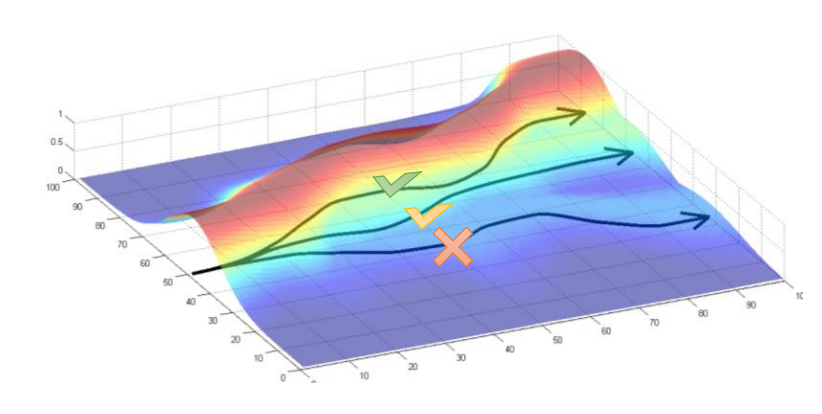
\includegraphics[scale=0.5]{figures/trajheat.png}
    \caption{More rewarding trajectories are more probable.}
    \label{fig:trajheat}
\end{figure}

\section{Partial Observability}
Can we use the policy gradient on a Partially Observed Markov Decision Process (POMDP)? The short answer is Yes. Why? Recall (yet again) the policy gradient expression:

$$\nabla_\theta J(\theta) \simeq \frac{1}{N}\sum_{i=1}^N\left(\sum_{t=1}^T\nabla_\theta \log\pi_\theta(a_{i,t}|s_{i,t})\right)\left(\sum_{t=1}^T r(s_{i,t},a_{i,t})\right)$$

In this expression, we do not even have the transition function in it. Long story short, the Markovian property is not actually used! So we can use policy gradient on a POMDP without any modification except instead of $s_t$, we use $o_t$.

Note that we do not care about what the state actually is. Any Non-Markovian proces can be made Markovian by setting the state as the whole history. 

\section{Disadvantages of the Policy Gradient}
Recall the intuition behind the policy gradient update: we make trajectories with more reward more probable. Let's consider the following scenario: say two trajectories have similar positive rewards, while another trajectory has a low, negative reward. Then policy gradient is going to assign zero to low probability to the third reward, and high probabilities to the other two. Now imagine we add a large constant number to our reward function, and apparently it does not change the relative relation between different trajectories' rewards because we are only adding in a constant. Now the negative reward becomes positive, and policy gradient is likely to spread out the likelihood for the three trajectories since all three rewards are positive now. This is bad because our reward does not change at all in fact, but after adding in a constant, the distribution of policy gradient changed substantially. 

Therefore, we need to come up with some methods to reduce the variance introduced in the policy gradients. 
\section{Reducing Policy Gradients Variance using Baselines}
\subsection{Causality}
One simple fix for high variance is to use the fact of causality: policy at time $t'$ cannot affect reward at $t$ if $t<t'$. This simple commonsensical idea allows us to discard some operands in the summation:
$$\nabla_\theta J(\theta) \simeq \frac{1}{N}\sum_{i=1}^N\left(\sum_{t=1}^T\nabla_\theta \log\pi_\theta(a_{i,t}|s_{i,t})\right)\left(\sum_{t'=t}^T r(s_{i,t'},a_{i,t'})\right)$$
and we define the second item in the summation as the ``reward-to-go''. Notice that in the reward-to-go term, we start the summation from time $t$ instead of 1, by causality. The idea is that we are multiplying the likelihood by smaller numbers due to the reduction of the summation term, so we can reduce the variance to some extent.
\subsection{Baselines}
Another common approach is to use baselines. By baselines, we mean that instead of making all high-reward trajectories more likely, we only make trajectories \textbf{better than average} more likely. So naturally, we define a baseline $b$ as the average reward:
$$b = \frac{1}{N} \sum_{i=1}^Nr(\tau)$$
Incorporating the baseline $b$ into our original policy gradient expression:
$$\nabla_\theta J(\theta) \simeq \frac{1}{N}\sum_{i=1}^N \nabla_\theta \log\pi_\theta(\tau)\left[r(\tau)-b\right]$$
But, are we allowed to that? Yes, in fact, we can show that the expectation is the same with baseline $b$. To show this, we can express the expectation of baseline as:
\begin{align*}
\mathbb{E}\left[\nabla_\theta\log \pi_\theta(\tau)b\right]&=
\int \pi_\theta(\tau)\nabla \log\pi_\theta(\tau)b\;d\tau\\
&=\int \nabla_\theta \pi_\theta(\tau)b\;d\tau\\
&=b\nabla_\theta\int\pi_\theta(\tau)\;d\tau\\
&=b\nabla_\theta 1\\
&=0
\end{align*}
Therefore, by subtracting a baseline, our policy gradient is still unbiased in expectation!
\subsection{Analyzing the Variance with Baselines}
Let us explicitly write down the variance of the policy gradient. Recall the definition of variance:
$$\mathrm{Var}[x] = \mathbb{E}[x^2]-\mathbb{E}[x]^2$$
And the policy gradient with baselines is written as:
$$\nabla_\theta J(\theta) \simeq \mathbb{E}_{\tau\sim\pi_\theta(\tau)}\left[\nabla_\theta \log\pi_\theta(\tau)\left(r(\tau)-b\right)\right]$$
Therefore, the variance of the policy gradient can be written as follows:
$$\mathrm{Var} = \mathbb{E}_{\tau\sim\pi_\theta(\tau)}\left[\left(\nabla_\theta \log\pi_\theta(\tau)\left(r(\tau)-b\right)\right)^2\right] - \mathbb{E}_{\tau\sim\pi_\theta(\tau)}\left[\nabla_\theta \log\pi_\theta(\tau)\left(r(\tau)-b\right) \right]^2$$
Note that in the second expectation term of variance, it can be equivalently written as $\mathbb{E}_{\tau\sim\pi_\theta(\tau)}\left[\nabla_\theta \log\pi_\theta(\tau)r(\tau) \right]^$ since baselines are unbiased in expectation.

Now we have an expression of variance with respect to baseline $b$, we can calculate the optimal $b$ that minimizes the variance by setting the gradient of variance to 0:
\begin{align*}
    \frac{d\mathrm{Var}}{db} &= \frac{d}{db}\mathbb{E}\left[g(\tau)^2(r(\tau)-b)^2\right]\\ &=\frac{d}{db}\mathbb{E}\left[g(\tau)^2r(\tau)^2\right] - 2\mathbb{E}\left[g(\tau)^2r(\tau)b\right] + b^2\mathbb{E}\left[g(\tau)^2\right]\\
    &=-2\mathbb{E}\left[ g(tau)^2r(\tau)\right]+2b\mathbb{E}\left[g(\tau)^2\right]\\
    &=0
\end{align*}
Solving the equation, we will have
$$b^{opt} = \frac{\mathbb{E}\left[g(\tau)^2r(\tau)\right]}{\mathbb{E}\left[g(\tau)^2\right]}$$
where $b^{opt}$ is the optimal baseline value for reducing the variance.

In practice, we just use the average reward for baseline. 

\section{On-Policy vs. Off-Policy}
We now introduce two concepts in RL: on-policy and off-policy. On-policy means that we learn only from using the current policy $\pi_\theta$, and off-policy means we learn also from other policies. Apparently, policy gradient is an on-policy method because $\nabla_\theta J(\theta) \simeq \mathbb{E}_{\tau\sim\pi_\theta(\tau)}\left[\nabla_\theta \log\pi_\theta(\tau)\left(r(\tau)-b\right)\right]$, and the expectation is taken under the current, known trajectory of interest. Therefore, every time we have a new policy, we need to use new samples. Since we are changing $\theta$, $\pi_\theta$ also changes overtime in policy gradient. One can imagine that this is extremely inefficient in neural networks, because in a neural network, $\theta$ only changes a little and the overhead for changing the policy is large.

One solution is to use off-policy learning.

\subsection{Off-policy Learning and Importance Sampling}
We first introduce an important technique called importance sampling. Given a distribution $p(x)$, how do we calculate the expectation from samples from another distribution $q(x)$? This is the idea of importance sampling, by using an importance ratio, we can calculate the expectation from another distribution, this enabling to learn off-policy. 

In importance sampling:
\begin{align*}
    \mathbb{E}_{x\sim p(x)}\left[f(x)\right] &= \int p(x)f(x)\;dx\\
    &=\int \frac{q(x)}{p(x)}f(x)\;dx\\
    &=\mathbb{E}_{x\sim q(x)}\left[\frac{p(x)}{q(x)}f(x)\right]
\end{align*}

Then we can plug it into the off-policy policy gradient. Say we have a trained policy $\pi_\theta(\tau)$, and we have samples from another policy $\Bar{\pi}(\tau)$, we can use the samples from $\Bar{\pi}(\tau)$ to calculate $J(\theta)$ function using importance sampling:
\begin{align*}
    J(\theta) &= \mathbb{E}_{\tau\sim\pi_\theta(\tau)}\left[r(\tau)\right]\\
    &= \mathbb{E}_{\tau\sim\Bar{\pi}(\tau)}\left[ \frac{\pi_\theta(\tau)}{\Bar{\pi}(\tau)} r(\tau)\right]
\end{align*}
Now we want to look closely at the importance ratio. Recall that $\pi_\theta(\tau) = p(s_1)\prod_{t=1}^T\pi_\theta(a_t|s_t)p(s_{t+1}|s_t,a_t)$. Then we can simplify the ratio in the following way:
\begin{align*}
\frac{\pi_\theta(\tau)}{\Bar{\pi}(\tau)} &=\frac{p(s_1)\prod_{t=1}^T\pi_\theta(a_t|s_t)p(s_{t+1}|s_t,a_t)}{p(s_1)\prod_{t=1}^T\Bar{\pi}(a_t|s_t)p(s_{t+1}|s_t,a_t)}\\
&= \frac{\prod_{t=1}^T\pi_\theta(a_t|s_t)}{\prod_{t=1}^T\Bar{\pi}(a_t|s_t)}
\end{align*}
\subsection{Deriving Policy Gradient with Importance Sampling}
It turns out that we can recover the original policy gradient theorem using off-policy learning using importance sampling. Recall the objective of RL as defined in the first chapter:
$$\theta^* = \argmaxA_\theta J(\theta)$$
and we defined $J(\theta)$ as $J(\theta) = \mathbb{E}_{\tau\sim\pi_\theta(\tau)}\left[r(\tau)\right]$. Now if we want to estimate $J$ with some new parameter $\theta'$, we can use importance sampling as discussed above:
$$J(\theta') = \mathbb{E}_{\tau\sim\pi_\theta(\tau)}\left[\frac{\pi_{\theta'}(\tau)}{\pi_\theta(\tau)}r(\tau)\right]$$
then we take the gradient as:
$$\nabla_{\theta'}J(\theta') &= 
    \mathbb{E}_{\tau\sim\pi_\theta(\tau)}\left[\frac{\nabla_{\theta'}\pi_{\theta'}(\tau)}{\pi_\theta(\tau)}r(\tau)\right]\\
    &=\mathbb{E}_{\tau\sim\pi_\theta(\tau)}\left[\frac{\pi_{\theta'}(\tau)}{\pi_\theta(\tau)}\nabla_{\theta'}\log \pi_{\theta'}(\tau)r(\tau)\right]
$$

Now if we estimate it locally, by setting $\theta = \theta'$, then we will cancel out the importance ratio, ending up with $\mathbb{E}_{\tau\sim\pi_\theta(\tau)}\left[\nabla_{\theta'}\log \pi_{\theta'}(\tau)r(\tau)\right]$.

\section{First Order Approximation for Importance Sampling}
Now we focus on the cases where we do not use local approximation, when $\theta \neq \theta'$.
\begin{align*}
    J(\theta') &= \mathbb{E}_{\tau\sim\pi_\theta(\tau)}\left[r(\tau)\right]\\
    \nabla_{\theta'}J(\theta')&=\mathbb{E}_{\tau\sim\pi_\theta(\tau)}\left[\frac{\pi_{\theta'}(\tau)}{\pi_\theta(\tau)}\nabla_{\theta'}\log\pi_{\theta'}(\tau)r(\tau)\right]\\
    &= \mathbb{E}_{\tau\sim\pi_\theta(\tau)}\left[  \left(  \frac{\prod_{t=1}^T\pi_{\theta'}(a_t|s_t)}{\prod_{t=1}^T\pi_{\theta}(a_t|s_t)} \right)\left( \sum_{t=1}^T\nabla_{\theta'}\log\pi_{\theta'}(a_t|s_t)  \right)\left(\sum_{t=1}^Tr(s_t,a_t)\right)  \right]
\end{align*}
Now there is a problem in the equation. Note that the ratio of the two products can be very small or very big if $T$ is big, thus increasing the variance. To alleviate the issue, one can make use of causality as we discussed before:
\begin{align*}
    \nabla_{\theta'}J(\theta')&= \mathbb{E}_{\tau\sim\pi_\theta(\tau)}\left[  \left(  \frac{\prod_{t=1}^T\pi_{\theta'}(a_t|s_t)}{\prod_{t=1}^T\pi_{\theta}(a_t|s_t)} \right)\left( \sum_{t=1}^T\nabla_{\theta'}\log\pi_{\theta'}(a_t|s_t)  \right)\left(\sum_{t=1}^Tr(s_t,a_t)\right)  \right]\\
    &=\mathbb{E}_{\tau\sim\pi_\theta(\tau)}\left[  \sum_{t=1}^T\nabla_{\theta'}\log\pi_{\theta'}(a_t|s_t) \left(\prod_{t'=1}^T \frac{\pi_{\theta'}(a_{t'}|s_{t'}) }{\pi_{\theta}(a_{t'}|s_{t'})}\right)    \left(  \sum_{t'=t}^Tr(s_{t'},a_{t'})\left(  \prod_{t'' = t}^{t'}\frac{\pi_{\theta'}(a_{t''}|s_{t''}) }{\pi_{\theta}(a_{t''}|s_{t''})} \right)    \right)\right]
\end{align*}
Here we used the fact of causality that future actions don't affect the current weight. Also note that the last ratio of products can be deleted, and we essentially get the policy iteration algorithm, which we will discuss in later chapters. 

So when we delete the last weight, we end up having
$$\nabla_{\theta'}J(\theta')= \mathbb{E}_{\tau\sim\pi_\theta(\tau)}\left[   \sum_{t=1}^T\nabla_{\theta'}\log\pi_{\theta'}(a_t|s_t)    \left(\prod_{t'=1}^T \frac{\pi_{\theta'}(a_{t'}|s_{t'}) }{\pi_{\theta}(a_{t'}|s_{t'})}\right)\left(  \sum_{t'=t}^Tr(s_{t'},a_{t'})\right)\right]$$
The product of ratio is again exponential in $T$, so we may have high variance. 

Recall on-policy policy gradient:
$$\nabla_{\theta}J(\theta) \simeq \frac{1}{N} \sum_{i=1}^T \sum_{t=1}^T\nabla_\theta \log \pi_\theta(a_{i,t}|s_{i,t})\hat{Q}_{i,t}$$
Similarly in off-policy policy gradient:
\begin{align*}
    \nabla_{\theta'}J(\theta') &= \frac{1}{N} \sum_{i=1}^T \sum_{t=1}^T   \frac{\pi_{\theta'}(s_{i,t},a_{i,t})}{\pi_{\theta}(s_{i,t},a_{i,t})}\nabla_{\theta'} \log \pi_{\theta'}(a_{i,t}|s_{i,t})\hat{Q}_{i,t}\\
    &= \frac{1}{N} \sum_{i=1}^T \sum_{t=1}^T \frac{\pi_{\theta'}(s_{i,t})}{\pi_{\theta}(s_{i,t})}\frac{\pi_{\theta'}(s_{i,t}|a_{i,t})}{\pi_{\theta}(s_{i,t}|a_{i,t})}\nabla_{\theta'} \log \pi_{\theta'}(a_{i,t}|s_{i,t})\hat{Q}_{i,t}
\end{align*}
In later chapters, we can see that we can pretty much ignore the first states priors ratio.